\documentclass{article}
\usepackage{graphicx}
\usepackage{hyperref}
\usepackage{framed}
\usepackage{xcolor}

\hypersetup{
    colorlinks=true,
    linkcolor=blue,
    filecolor=magenta,
    urlcolor=cyan,
    pdftitle={Overleaf Example},
    pdfpagemode=FullScreen,
    }
\begin{document}

\includegraphics[width=0.3\textwidth]{esi.png}
\thispagestyle{empty}
\begin{center}
    \vspace*{3cm}
    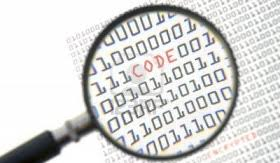
\includegraphics[width=1\textwidth]{ste.jpeg}
    \Huge
    \hrule
    \vspace{0.5cm}
    stéganographie d'image bmp
    \vspace{0.5cm}
    \hrule
    \vspace{1cm}
    \Large
    Vivace Fouefack \\

\end{center}
\newpage
\renewcommand{\contentsname}{Table des matières}
\tableofcontents
\newpage
\section{Introduction}

\subsection{Définition de la stéganographie}
La stéganographie est l'art de dissimuler des informations dans des supports tels que des images, des vidéos ou des fichiers audio, de manière à ce que la présence de ces données soit imperceptible. Dans cette étude, nous allons explorer la stéganographie appliquée aux images BMP (Bitmap).
\subsection{Objectifs et applications de la stéganographie}
La stéganographie, en tant que discipline spécialisée dans la dissimulation d'informations, poursuit plusieurs objectifs et trouve des applications diverses. Ces objectifs et applications démontrent l'importance croissante de la stéganographie dans des contextes variés.
\subsubsection{Objectifs de la stéganographie}
\bfseries Confidentialité des Données\normalfont : L'objectif principal de la stéganographie est de garantir la confidentialité des données. En dissimulant des informations sensibles au sein d'autres supports, elle vise à empêcher la détection ou l'interception par des tiers non autorisés en intégrant des messages au sein de supports apparemment ordinaires. Cela peut être crucial dans des contextes tels que la sécurité nationale, la défense militaire, ou même la protection des informations commerciales confidentielles.

\bfseries Contournement de la Détection\normalfont : Contrairement à la cryptographie qui vise à rendre les données illisibles, la stéganographie se concentre sur le fait de rendre les données invisibles. Cela permet d'éviter la détection, offrant ainsi un niveau supplémentaire de sécurité.

\subsubsection{Applications de la Stéganographie}
\bfseries Sécurité des Communications\normalfont : La stéganographie trouve des applications dans la sécurité des communications, où la confidentialité des informations échangées est cruciale. Elle est utilisée pour protéger les communications gouvernementales, militaires et diplomatiques.

\bfseries Protection des Droits d'Auteur\normalfont : Dans le domaine numérique, la stéganographie est utilisée pour protéger les droits d'auteur en intégrant des marques invisibles dans les médias, permettant ainsi de tracer l'origine des œuvres et de détecter les utilisations non autorisées.

\bfseries Sécurité Informatique\normalfont : En informatique, la stéganographie peut être utilisée pour dissimuler des informations d'identification ou des codes malveillants, rendant ainsi plus difficile la détection par les logiciels antivirus.
\section{Structure du format BMP}
Le format BMP (Bitmap) est un format de fichier d'image bitmap largement utilisé pour stocker des images sur les systèmes d'exploitation Windows. La structure du format BMP est composée de différentes parties, chacune ayant un rôle spécifique dans la définition et la représentation de l'image.
\subsection{En-tête du fichier (File Header)}
L'en-tête du fichier est la première partie du format BMP et fournit des informations de base sur le fichier image. Il est structuré comme suit :\\

\bfseries Type de Fichier (2 octets)\normalfont : Identifie le type de fichier, généralement défini à "BM" (4D42) pour Bitmap.\\

\bfseries Taille du Fichier (4 octets) \normalfont : Indique la taille totale du fichier en octets.\\

\bfseries Réserve (4 octets)\normalfont : Réservé à des fins spécifiques, généralement mis à zéro.\\

\bfseries Offset de l'Image (4 octets) \normalfont : Définit l'offset (décalage) en octets depuis le début du fichier jusqu'au début des données de l'image.

\subsection{En-tête de l'image (Bitmap Information Header)}
L'en-tête de l'image suit immédiatement l'en-tête du fichier et contient des informations spécifiques à l'image. Les principaux champs sont :

\bfseries Taille de l'En-tête (4 octets)\normalfont : Indique la taille de l'en-tête de l'image.

\bfseries Largeur (4 octets) \normalfont : Définit la largeur de l'image en pixels.

\bfseries Hauteur (4 octets) \normalfont : Indique la hauteur de l'image en pixels.

\bfseries  Nombre de Plans (2 octets)\normalfont : Spécifie le nombre de plans de couleur, généralement mis à 1.

\bfseries Profondeur de Couleur (2 octets)\normalfont : Indique la profondeur de couleur en bits par pixel. Le format BMP permet de prendre en charge différentes profondeurs de bits pour représenter la couleur des pixels dans une image. parmi ces pronfondeurs, nous avons:
\begin{itemize}
\item BMP 1-bit: Permet de représenter deux couleurs (généralement noir et blanc) en utilisant un seul bit par pixel. Chaque pixel peut être soit allumé (1) soit éteint (0).

\item BMP 4-bit: Permet de représenter jusqu'à 16 couleurs en utilisant 4 bits par pixel. Cela est utilisé dans des images avec une palette de couleurs limitée.

\item BMP 8-bit: Permet de représenter jusqu'à 256 couleurs en utilisant 8 bits par pixel. Comme le BMP 4-bit, cela est utilisé avec une palette de couleurs.

\item BMP 16-bit: Utilise 16 bits par pixel pour représenter des images en couleur. Il peut représenter une gamme plus large de couleurs que les versions précédentes, mais la précision des couleurs est limitée par rapport aux formats avec plus de bits.

\item BMP 24-bit: Représente la couleur avec 24 bits par pixel, permettant une représentation plus précise des couleurs. Chaque pixel est représenté par trois canaux de 8 bits (rouge, vert, bleu).

\item BMP 32-bit: Utilise 32 bits par pixel, souvent avec une composante alpha en plus des canaux rouge, vert et bleu. La composante alpha permet de représenter la transparence.
\end{itemize}
\bfseries Compression (4 octets)\normalfont : Spécifie le type de compression utilisé pour l'image s'il y en a (la compression RLE est généralememt utiliser).

\bfseries Taille de l'Image (4 octets)\normalfont : Indique la taille totale de l'image en octets.

\subsection{Palette de Couleurs (Color Palette)}
La palette de couleurs est utilisée pour définir les couleurs disponibles dans l'image, en particulier dans les images avec une profondeur de couleur inférieure à 24 bits par pixel. La palette est facultative pour les images TrueColor (24 bits par pixel).
\subsection{Tableau des Pixels (Pixel Array)}
Le tableau des pixels contient les données réelles de l'image, où chaque pixel est représenté par une série de bits. La disposition des bits dépend de la profondeur de couleur définie dans l'en-tête de l'image. Pour les images TrueColor, chaque pixel peut être composé de trois composantes : rouge, vert et bleu (RVB), tandis que les images à palette utiliseront des indices de couleur pour faire référence à la palette. c'est à ce niveau que nous allons agir pour dissimuler les données dans l'image.

\section{Cas pratique de dissimulation de Données dans une Image}
Après avoir examiné attentivement la structure du format BMP, nous allons désormais mettre en pratique la manipulation des données d'une image. À cette fin, nous opterons pour le format BMP 24 bits en raison de sa large gamme de couleurs, offrant ainsi la capacité de dissimuler une quantité importante de données.

\subsection{Manipulation des pixels}
Un pixel (contraction des termes anglais "picture" et "element") est l'unité élémentaire de base dans une image numérique. Il représente un point ou un élément discret dans une grille, formant ainsi la structure de base d'une image matricielle. Chaque pixel de l'image est associé à une couleur spécifique, déterminée par le pourcentage de la composante rouge, verte et le bleu.
\begin{figure}[h]
  \centering
  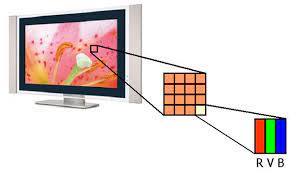
\includegraphics[width=0.9\textwidth]{pixel.jpeg}
  \caption{Représention d'un pixel.}
\end{figure}

La résolution d'une image est souvent exprimée en termes du nombre total de pixels dans ses dimensions. Par exemple, une image de 1920x1080 a une résolution de 1920 pixels en largeur et 1080 pixels en hauteur.

Dans une image BMP, le tableau de pixels est représenté en mémoire de manière linéaire, sous forme de tableau à une dimension. Cela signifie que les valeurs des pixels sont stockées consécutivement dans la mémoire, sans distinction entre les lignes et les colonnes de l'image. Etant donné que nous travaillons avec une image 2D, la formule utilisée pour calculer l'indice d'un pixel dans ce tableau à une dimension à partir des coordonnées (X, Y) est la suivante :\
\bfseries \begin{center}
    index = Y * width + X \normalfont où :
\end{center}
\begin{itemize}
\item \bfseries index \normalfont est l'indice dans le tableau à une dimension.
\item \bfseries Y \normalfont est la coordonnée en hauteur (ligne) du pixel.
\item \bfseries X \normalfont  est la coordonnée en largeur (colonne) du pixel.
\item \bfseries width \normalfont  est la largeur de l'image en pixels.
\end{itemize}

\normalfont En utilisant cette formule, nous allons accéder à chaque pixel dans le tableau à une dimension en fonction des coordonnées (X, Y) de l'image.

\begin{table}[h]
  \centering
  \begin{tabular}{|c|c|c|c|}
    \hline
    \textbf{Pixel} & \textbf{Rouge (8 bits)} & \textbf{Vert (8 bits)} & \textbf{Bleu (8 bits)} \\
    \hline
    (0, 0) & 11111111 & 11111111 & 11111111 \\
    (0, 1) & 00000000 & 11111111 & 00000000 \\
    (0, 2) & 00000000 & 00000000 & 11111111 \\
    (0, 3) & 11111111 & 11111111 & 11111111 \\
    \hline
    (1, 0) & 00000000 & 11111111 & 11111111 \\
    (1, 1) & 11111111 & 00000000 & 11111111 \\
    (1, 2) & 11111111 & 11111111 & 00000000 \\
    (1, 3) & 10000000 & 10000000 & 10000000 \\
    \hline
    (2, 0) & 00000000 & 00000000 & 00000000 \\
    (2, 1) & 10000000 & 00000000 & 00000000 \\
    (2, 2) & 00000000 & 10000000 & 00000000 \\
    (2, 3) & 00000000 & 00000000 & 10000000 \\
    \hline
    (3, 0) & 10000000 & 00000000 & 10000000 \\
    (3, 1) & 11111111 & 10100101 & 00000000 \\
    (3, 2) & 11111111 & 10110110 & 11000001 \\
    (3, 3) & 01000000 & 11100000 & 11010000 \\
    \hline
  \end{tabular}
  \caption{Tableau des pixels d'une image BMP 24 bits}
  \label{}
\end{table}
Chaque composant peut être représenté par 8 bits (1 octet), où le bit le plus à gauche (le septième bit) est désigné comme le bit de poids fort (Most Significant Bit), et le bit le plus à droite (le premier bit) est désigné comme le bit de poids faible (Least Significant Bit).
\begin{figure}[h]
  \centering
  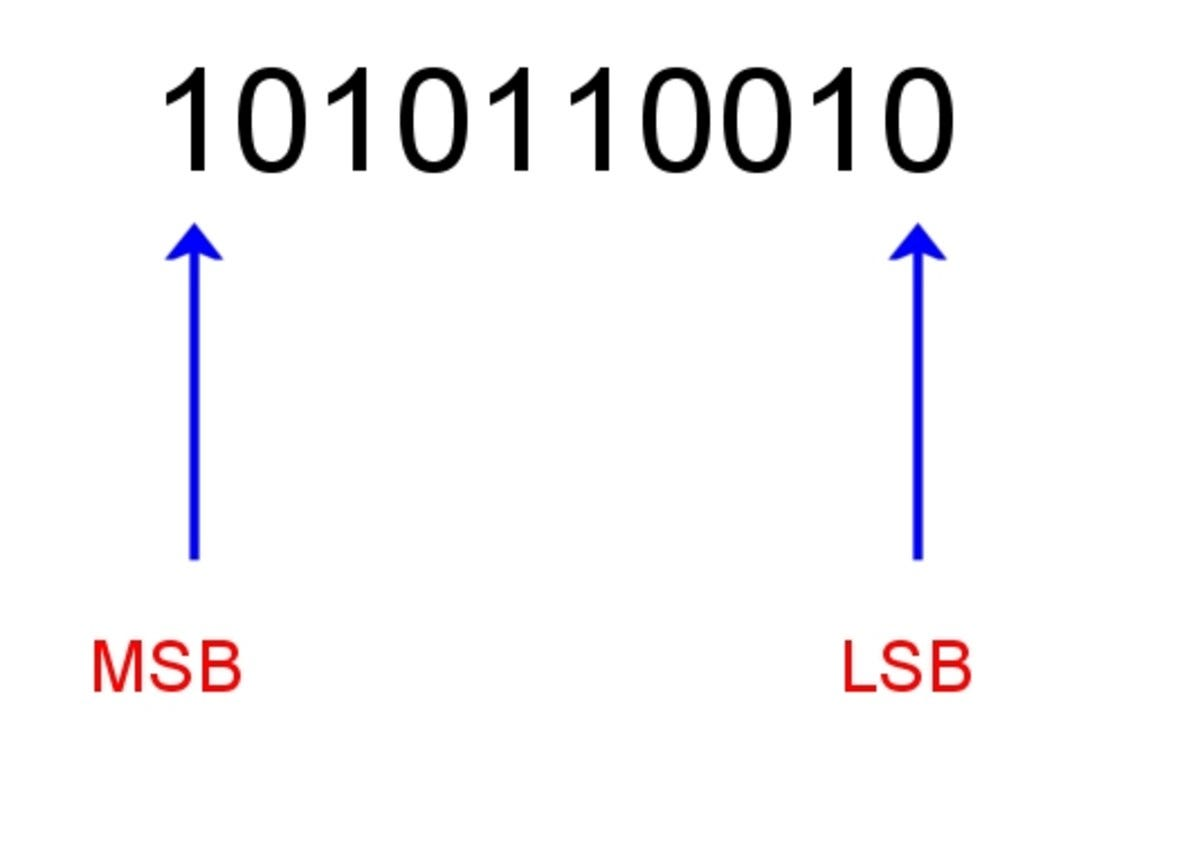
\includegraphics[width=0.6\textwidth]{bit.jpg}
  \caption{MSB et LSB.}
\end{figure}\\
En raison de la pondération décroissante des bits dans la représentation binaire, la modification du bit de poids faible (LSB) d'un octet aura un impact minimal sur la valeur numérique de cet octet, et par conséquent, un impact visuel négligeable. Nous allons exploiter cette propriété afin de dissimuler les information dans une image.
\begin{figure}[h]
  \centering
  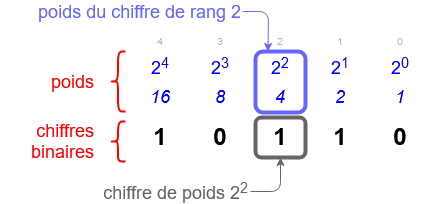
\includegraphics[width=0.7\textwidth]{pon.png}
  \caption{Pondération binaire.}
\end{figure}

\subsection{Dissimulation d'un fichier texte dans une image}
Dans cette section, nous allons aborder le traitement pixel par pixel, ce qui nous permettra de manipuler les composantes de couleur de chaque pixel de manière individuelle. L'objectif principal est de remplacer les bits de poids faible des composantes de couleur d'un pixel par les bits provenant de l'extraction des bits du contenu du fichier texte que nous souhaitons dissimuler.

\subsubsection{Extraction des bits du texte}
À chaque caractère du fichier texte correspond l'extraction d'une séquence binaire. Chaque caractère est représenté par une série de 8 bits.\\\\
Exemple :
\begin{center}
    \textbf{Secret.txt}
\end{center}
\begin{framed}
Le noyau Linux est le cœur du système d'exploitation Linux. Il s'agit d'un noyau de système d'exploitation de type UNIX, initialement créé par Linus Torvalds en 1991. Le noyau Linux est open source et distribué sous les termes de la licence GPL (GNU General Public License).
Le noyau Linux joue un rôle crucial dans le fonctionnement du système d'exploitation. Il gère les ressources du matériel, offre des services système de base, et assure la communication entre les logiciels applicatifs et le matériel.
\end{framed}
\newpage
\begin{center}
    \textbf{hide.c}
\end{center}
\begin{framed}
\begin{verbatim}
#include<stdio.h>
#include <stdint.h>

char * textInBinary(const char * text) {
    int size = 0;
    while (text[size]) {
        size++;
    }

    char * binaryText = (char *)malloc(len * 8 + 1);
    if (binaryText == NULL) {
        printf("Erreur d'allocation mémoire.\n");
        exit(1);
    }

    int index = 0;
    for (int i = 0; i < size; ++i) {
        for (int j = 7; j >= 0; --j) {
            binaryText[index++] = ((text[i] >> j) & 1) + '0';
        }
    }
    binaryText[index] = '\0';
    return binaryText;
}

int main(int argc, char *argv[]) {
    printf("%s",textInBinary("texte à extraire ici"));
    return 0;
}
\end{verbatim}
\end{framed}

Résultat :\\01001100 01100101 00100000 01101110 01101111 01111001 01100001 01110101 00100000 01001100 01101001 01101110 01110101 01111000 00100000 01100101 01110011 01110100 00100000 01101100 01100101 00100000 01100011  01101111 01100101 01110010 00100000 01100100 01110101 00100000 01110011 01111001 01110011 01110100 01100101 01101101 01100101 00100000 01100100  01110010 01100011 01100101 01110011 01110011 01100101 01110011 01110011 01101111 01110011 01110011 01101111 01101111 01110111 01100001 01101010 01101111 01110111 01100111 01100101 01110011 01110100 01101011 01110011 01110111 01101111 01110111 01101111 01110111 01110111 01110111 01110111 01110111 01110111 01110111 ...\\

\subsubsection{Accès aux pixels et remplacement des bits}
En fonction de la taille du texte à dissimuler, nous allons parcourir le tableau des pixels de l'image et pour chaque composante de couleur (R,V,B) d'un pixel, remplacez le bit de poids faible par les bits extraits du fichier texte en utilisant des opérations de masquage et de décalage. Cette opération est cruciale pour garantir une dissimulation efficace des données tout en minimisant l'impact visuel sur l'image.Les codes suivant présentent une implémentation simplifiée du processus d'accès aux pixels et de remplacement des bits de poids faible :
\begin{center}
    \textbf{bmp.c}
\end{center}
\begin{framed}
\begin{verbatim}
#ifndef BMP_H
#define BMP_H
#include <stdint.h>
typedef struct {
    unsigned short type;
    unsigned int size;
    unsigned short reserved1;
    unsigned short reserved2;
    unsigned int offsetbits;
} __attribute__ ((packed)) bmpheader;

typedef struct {
    unsigned int headersize;
    int width;
    int height;
    unsigned short planes;
    unsigned short bitcount;
    unsigned int compression;
    unsigned int sizeimage;
    int xpelspermeter;
    int ypelspermeter;
    unsigned int colorsused;
    unsigned int colorsimportant;
    unsigned char * palette;
    unsigned char * pixels;
} __attribute__ ((packed)) bmpinfo;
#endif
\end{verbatim}
\end{framed}
\newpage
\begin{center}
    \textbf{hide.c}
\end{center}
\begin{framed}
\begin{verbatim}
#include<stdio.h>
#include <stdint.h>
#include<stdlib.h>
#include <fcntl.h>
#include <unistd.h>
#include "bmp.h"

void hideTextInImage(){
FILE * img =fopen("papillon6136.bmp", "rb");
FILE * textFile = fopen("secret.txt", "rb");
bmpheader header;
bmpinfo info;
fread(&header, sizeof(header), 1, img);
fread(&info, sizeof(info), 1, img);
info.pixels = (unsigned char *)malloc(info.sizeimage);
fread(info.pixels, 1, info.sizeimage, img);
fclose(img);
int binaryIndex = 0;
for (int y = 0; y < info.height; ++y) {
for (int x = 0; x < info.width; ++x) {
    int pixelIndex = (y * info.width + x) * 3;
    for (int component = 0; component < 3; component++) {
        if (binaryIndex >= textFileSize)
            break;
        char pixelComponent=info.pixels[pixelIndex + component];
        //binaryText est le tableau de caractère qui contient
        //tous les bits extraits du texte.
        char textBit=binaryText[binaryIndex ];
        info.pixels[pixelIndex + component] =
        (pixelComponent & 0xFE) | (textBit - '0');
        binaryIndex++;
    }
    if (binaryIndex >= textFileSize)
        break;
}
}
}

\end{verbatim}
\end{framed}

Après cette opération, le fichier "secret.txt" est inséré dans l'image et notre tableau de pixels vu précédemment devient :

\newpage

\begin{table}[h]
  \centering
  \begin{tabular}{|c|c|c|c|}
    \hline
    \textbf{Pixel} & \textbf{Rouge (8 bits)} & \textbf{Vert (8 bits)} & \textbf{Bleu (8 bits)} \\
    \hline
    (0, 0) & 1111111\textcolor{red}{0} & 1111111\textcolor{red}{1} & 1111111\textcolor{red}{0} \\
    (0, 1) & 0000000\textcolor{red}{0} & 1111111\textcolor{red}{1} & 0000000\textcolor{red}{1} \\
    (0, 2) & 0000000\textcolor{red}{1} & 0000000\textcolor{red}{1} & 1111111\textcolor{red}{0} \\
    (0, 3) & 1111111\textcolor{red}{0} & 1111111\textcolor{red}{1} & 1111111\textcolor{red}{0} \\
    \hline
    (1, 0) & 0000000\textcolor{red}{1} & 1111111\textcolor{red}{0} & 1111111\textcolor{red}{0} \\
    (1, 1) & 1111111\textcolor{red}{1} & 0000000\textcolor{red}{0} & 1111111\textcolor{red}{0} \\
    (1, 2) & 1111111\textcolor{red}{0} & 1111111\textcolor{red}{1} & 0000000\textcolor{red}{1} \\
    (1, 3) & 1000000\textcolor{red}{0} & 1000000\textcolor{red}{0} & 1000000\textcolor{red}{0} \\
    \hline
    (2, 0) & 0000000\textcolor{red}{0} & 0000000\textcolor{red}{1} & 0000000\textcolor{red}{1} \\
    (2, 1) & 1000000\textcolor{red}{1} & 0000000\textcolor{red}{0} & 0000000\textcolor{red}{0} \\
    (2, 2) & 0000000\textcolor{red}{1} & 1000000\textcolor{red}{1} & 0000000\textcolor{red}{0} \\
    (2, 3) & 0000000\textcolor{red}{1} & 0000000\textcolor{red}{1} & 1000000\textcolor{red}{1} \\
    \hline
    (3, 0) & 1000000\textcolor{red}{1} & 0000000\textcolor{red}{0} & 1000000\textcolor{red}{1} \\
    (3, 1) & 1111111\textcolor{red}{1} & 1010010\textcolor{red}{1} & 0000000\textcolor{red}{1} \\
    (3, 2) & 1111111\textcolor{red}{0} & 1011011\textcolor{red}{0} & 1100000\textcolor{red}{1} \\
    (3, 3) & 0100000\textcolor{red}{0} & 1110000\textcolor{red}{1} & 1101000\textcolor{red}{1} \\
    \hline
  \end{tabular}
  \caption{Tableau des pixels contenent le fichier secret}
  \label{}
\end{table}

\subsection{Extraction d'un fichier texte caché dans une image}
Cette opération d'extraction est l'inverse du processus de dissimulation.
\subsubsection{Extraction des bits de poids faible}
Nous allons parcourir le tableau des pixels de l'image en fonction de la taille des données cachées pour extraire le bit de poids faible de chaque composant de couleur (R,V,B). Ces bits extraits sont en suite rassemblés pour former une séquence binaire.
\subsubsection{Reconstruction du fichier texte}
La séquence binaire obtenue est regroupé en 8 bits (1 octet). Chaque groupe correspond à un caractère dans le texte. En regroupant ces caractères obtenus, on reconstruit le fichier texte original qui avait été dissimulé dans l'image. Illustrons cette opération à l'aide du code simplifié suivant :
\newpage
\begin{center}
    \textbf{extract.c}
\end{center}
\begin{framed}
\begin{verbatim}
void extractTextToFile(int textFileSize) {
FILE *img = fopen("imageOutput.bmp", "rb");
bmpheader header;
bmpinfo info;
fread(&header, sizeof(header), 1, img);
fread(&info, sizeof(info), 1, img);
info.pixels = (unsigned char *)malloc(info.sizeimage);
fread(info.pixels, 1, info.sizeimage, img);
fclose(img);
FILE * outputTextFile = fopen("extractFile", "wb");

int binaryIndex = 0;
char currentByte = 0;
int bitCount = 0;
for (int y = 0; y < info.height; ++y) {
for (int x = 0; x < info.width; ++x) {
    int pixelIndex = (y * info.width + x) * 3;
    for (int component = 0; component < 3; ++component) {
        if (binaryIndex >= textFileSize)
            break;
        char pixelComponent=info.pixels[pixelIndex + component];
        char textBit = (pixelComponent & 0x01) + '0';
        currentByte = (currentByte << 1) | (textBit - '0');
        ++bitCount;
        if (bitCount == 8) {
            fputc(currentByte, outputTextFile);
            currentByte = 0;
            bitCount = 0;
        }
        ++binaryIndex;
    }
    if (binaryIndex >= textFileSize)
        break;
    }
}
fclose(outputTextFile);
}
\end{verbatim}
\end{framed}

\section{Observations}
Au cours de nos expérimentations approfondies dans le processus de dissimulation de données, une observation fascinante a été faite, soulevant des possibilités de dissimulation de quantité encore plus importante de données tout en préservant l'intégrité visuelle de l'image.
Cette observation concerne la capacité à remplacer non pas seulement le bit de poids faible, mais l'ensemble des quatre premiers bits de chaque composante de couleur (R,V,B).

Dans le processus de dissimulation de texte dans une image, l'utilisation de bit de poids faible est courante pour minimiser l'impact visuel. Cependant, ce qui a captivé notre attention, c'est la constatation que même en allant au-delà de la norme conventionnelle (le premier bit), et en remplaçant les quatre premiers bits, l'image résultante demeure visuellement inchangée pour l'observateur. Le code suivant permet d'illustrer ce concept en montrant comment les quatre premiers bits peuvent être modifiés sans altérer de manière significative l'apparence de l'image.
\begin{center}
    \textbf{hide.c}
\end{center}
\begin{framed}
\begin{verbatim}
#include<stdio.h>
#include <stdint.h>
#include<stdlib.h>
#include <fcntl.h>
#include <unistd.h>
#include "bmp.h"

void hideTextInImage(){
FILE * img =fopen("papillon6136.bmp", "rb");
FILE * textFile = fopen("secret.txt", "rb");
bmpheader header;
bmpinfo info;
fread(&header, sizeof(header), 1, img);
fread(&info, sizeof(info), 1, img);
info.pixels = (unsigned char *)malloc(info.sizeimage);
fread(info.pixels, 1, info.sizeimage, img);
fclose(img);
int binaryIndex = 0;
for (int y = 0; y < info.height; ++y) {
for (int x = 0; x < info.width; ++x) {
    int pixelIndex = (y * info.width + x) * 3;
    for (int component = 0; component < 3; component++) {
        if (binaryIndex >= textFileSize)
            break;
        char pixelComponent=info.pixels[pixelIndex + component];
        //binaryText est le tableau de caractère qui contient
        //tous les bits extraits du texte.
        char textBit=binaryText[binaryIndex ];
        info.pixels[pixelIndex + component] =
        (pixelComponent & 0xFE) | (textBit - '0');
        for(int position = 0; position <4 ; ++position){
            char textBit=binaryText[binaryIndex ];
            int mask = 1 << position;
            info.pixels[pixelIndex + component] =
            (pixelComponent &~mask)|((textBit-'0') << position);
            binaryIndex++;
        }
    }
    if (binaryIndex >= textFileSize)
        break;
}
}
}

\end{verbatim}
\end{framed}

\section{Conclusion}
Notre exploration de la stéganographie d'images BMP a révélé des techniques sophistiquées pour dissimuler des données tout en préservant l'apparence visuelle. En manipulant les bits de poids faible des composantes couleur des pixels, nous avons démontré une dissimulation efficace. Les observations suggèrent même la possibilité de remplacer jusqu'a quatre premiers bits sans altérer significativement l'image.

Ces résultats ouvrent des perspectives intéressantes pour dissimuler davantage de données tout en conservant l'intégrité visuelle. La stéganographie, avec ses multiples applications, se positionne comme un outil précieux pour la confidentialité des données, la sécurité des communications et la protection des droits d'auteur dans le domaine numérique.

\section{Références}
\href{https://cdnpdf.com/embed/53951-compressed-image-file-formats-jpeg-png-gif-xbm-bmp-by-john-miano}{Compressed File Formats de John Miano}\\
\href{https://en.wikipedia.org/wiki/BMP_file_format}{BMP file format}\\
\href{https://www.researchgate.net/publication/271863505_A_Survey_of_Image_Steganography_Techniques}{International Journal of Advanced Science and Technology Vol. 54,  May, 2013 }\\
\href{https://cdn.hackaday.io/files/274271173436768/Simplified%20Windows%20BMP%20Bitmap%20File%20Format%20Specification.htm}{Windows BMP Bitmap File Format Specification}

\end{document}

